\documentclass[twoside]{book}

% Packages required by doxygen
\usepackage{fixltx2e}
\usepackage{calc}
\usepackage{doxygen}
\usepackage[export]{adjustbox} % also loads graphicx
\usepackage{graphicx}
\usepackage[utf8]{inputenc}
\usepackage{makeidx}
\usepackage{multicol}
\usepackage{multirow}
\PassOptionsToPackage{warn}{textcomp}
\usepackage{textcomp}
\usepackage[nointegrals]{wasysym}
\usepackage[table]{xcolor}

% Font selection
\usepackage[T1]{fontenc}
\usepackage[scaled=.90]{helvet}
\usepackage{courier}
\usepackage{amssymb}
\usepackage{sectsty}
\renewcommand{\familydefault}{\sfdefault}
\allsectionsfont{%
  \fontseries{bc}\selectfont%
  \color{darkgray}%
}
\renewcommand{\DoxyLabelFont}{%
  \fontseries{bc}\selectfont%
  \color{darkgray}%
}
\newcommand{\+}{\discretionary{\mbox{\scriptsize$\hookleftarrow$}}{}{}}

% Page & text layout
\usepackage{geometry}
\geometry{%
  a4paper,%
  top=2.5cm,%
  bottom=2.5cm,%
  left=2.5cm,%
  right=2.5cm%
}
\tolerance=750
\hfuzz=15pt
\hbadness=750
\setlength{\emergencystretch}{15pt}
\setlength{\parindent}{0cm}
\setlength{\parskip}{3ex plus 2ex minus 2ex}
\makeatletter
\renewcommand{\paragraph}{%
  \@startsection{paragraph}{4}{0ex}{-1.0ex}{1.0ex}{%
    \normalfont\normalsize\bfseries\SS@parafont%
  }%
}
\renewcommand{\subparagraph}{%
  \@startsection{subparagraph}{5}{0ex}{-1.0ex}{1.0ex}{%
    \normalfont\normalsize\bfseries\SS@subparafont%
  }%
}
\makeatother

% Headers & footers
\usepackage{fancyhdr}
\pagestyle{fancyplain}
\fancyhead[LE]{\fancyplain{}{\bfseries\thepage}}
\fancyhead[CE]{\fancyplain{}{}}
\fancyhead[RE]{\fancyplain{}{\bfseries\leftmark}}
\fancyhead[LO]{\fancyplain{}{\bfseries\rightmark}}
\fancyhead[CO]{\fancyplain{}{}}
\fancyhead[RO]{\fancyplain{}{\bfseries\thepage}}
\fancyfoot[LE]{\fancyplain{}{}}
\fancyfoot[CE]{\fancyplain{}{}}
\fancyfoot[RE]{\fancyplain{}{\bfseries\scriptsize Generated by Doxygen }}
\fancyfoot[LO]{\fancyplain{}{\bfseries\scriptsize Generated by Doxygen }}
\fancyfoot[CO]{\fancyplain{}{}}
\fancyfoot[RO]{\fancyplain{}{}}
\renewcommand{\footrulewidth}{0.4pt}
\renewcommand{\chaptermark}[1]{%
  \markboth{#1}{}%
}
\renewcommand{\sectionmark}[1]{%
  \markright{\thesection\ #1}%
}

% Indices & bibliography
\usepackage{natbib}
\usepackage[titles]{tocloft}
\setcounter{tocdepth}{3}
\setcounter{secnumdepth}{5}
\makeindex

% Hyperlinks (required, but should be loaded last)
\usepackage{ifpdf}
\ifpdf
  \usepackage[pdftex,pagebackref=true]{hyperref}
\else
  \usepackage[ps2pdf,pagebackref=true]{hyperref}
\fi
\hypersetup{%
  colorlinks=true,%
  linkcolor=blue,%
  citecolor=blue,%
  unicode%
}

% Custom commands
\newcommand{\clearemptydoublepage}{%
  \newpage{\pagestyle{empty}\cleardoublepage}%
}

\usepackage{caption}
\captionsetup{labelsep=space,justification=centering,font={bf},singlelinecheck=off,skip=4pt,position=top}

%===== C O N T E N T S =====

\begin{document}

% Titlepage & ToC
\hypersetup{pageanchor=false,
             bookmarksnumbered=true,
             pdfencoding=unicode
            }
\pagenumbering{alph}
\begin{titlepage}
\vspace*{7cm}
\begin{center}%
{\Large Experimental Robotics Assignment 1 }\\
\vspace*{1cm}
{\large Generated by Doxygen 1.8.13}\\
\end{center}
\end{titlepage}
\clearemptydoublepage
\pagenumbering{roman}
\tableofcontents
\clearemptydoublepage
\pagenumbering{arabic}
\hypersetup{pageanchor=true}

%--- Begin generated contents ---
\chapter{Namespace Index}
\section{Packages}
Here are the packages with brief descriptions (if available)\+:\begin{DoxyCompactList}
\item\contentsline{section}{\hyperlink{namespacecommand__generation}{command\+\_\+generation} }{\pageref{namespacecommand__generation}}{}
\item\contentsline{section}{\hyperlink{namespacestate__behavior}{state\+\_\+behavior} }{\pageref{namespacestate__behavior}}{}
\end{DoxyCompactList}

\chapter{Hierarchical Index}
\section{Class Hierarchy}
This inheritance list is sorted roughly, but not completely, alphabetically\+:\begin{DoxyCompactList}
\item State\begin{DoxyCompactList}
\item \contentsline{section}{state\+\_\+behavior.\+Normal}{\pageref{classstate__behavior_1_1Normal}}{}
\item \contentsline{section}{state\+\_\+behavior.\+Play}{\pageref{classstate__behavior_1_1Play}}{}
\item \contentsline{section}{state\+\_\+behavior.\+Sleep}{\pageref{classstate__behavior_1_1Sleep}}{}
\end{DoxyCompactList}
\end{DoxyCompactList}

\chapter{Class Index}
\section{Class List}
Here are the classes, structs, unions and interfaces with brief descriptions\+:\begin{DoxyCompactList}
\item\contentsline{section}{\hyperlink{classstate__behavior_1_1Normal}{state\+\_\+behavior.\+Normal} \\*This class defines the state of the state machine corresponding to the robot randomly moving in the 2D plane }{\pageref{classstate__behavior_1_1Normal}}{}
\item\contentsline{section}{\hyperlink{classstate__behavior_1_1Play}{state\+\_\+behavior.\+Play} }{\pageref{classstate__behavior_1_1Play}}{}
\item\contentsline{section}{\hyperlink{classstate__behavior_1_1Sleep}{state\+\_\+behavior.\+Sleep} }{\pageref{classstate__behavior_1_1Sleep}}{}
\end{DoxyCompactList}

\chapter{File Index}
\section{File List}
Here is a list of all documented files with brief descriptions\+:\begin{DoxyCompactList}
\item\contentsline{section}{/home/rohit/\+Exp\+Robo\+Assignment/src/robot\+\_\+motion/src/\hyperlink{random__motion_8cpp}{random\+\_\+motion.\+cpp} }{\pageref{random__motion_8cpp}}{}
\end{DoxyCompactList}

\chapter{Namespace Documentation}
\hypertarget{namespacecommand__generation}{}\section{command\+\_\+generation Namespace Reference}
\label{namespacecommand__generation}\index{command\+\_\+generation@{command\+\_\+generation}}
\subsection*{Functions}
\begin{DoxyCompactItemize}
\item 
def \hyperlink{namespacecommand__generation_af7f8b77f85afe773fee4770435f86060}{main} ()
\begin{DoxyCompactList}\small\item\em the main function here published to rostopic. \end{DoxyCompactList}\end{DoxyCompactItemize}


\subsection{Detailed Description}
\begin{DoxyVerb}#   \file command_generation.py
#   \brief This file contains the command to call the robot for play behavior
#   \author Rohit Kumar
#   \version 0.2
#   \date 2020-11-13
#
\end{DoxyVerb}
 

\subsection{Function Documentation}
\mbox{\Hypertarget{namespacecommand__generation_af7f8b77f85afe773fee4770435f86060}\label{namespacecommand__generation_af7f8b77f85afe773fee4770435f86060}} 
\index{command\+\_\+generation@{command\+\_\+generation}!main@{main}}
\index{main@{main}!command\+\_\+generation@{command\+\_\+generation}}
\subsubsection{\texorpdfstring{main()}{main()}}
{\footnotesize\ttfamily def command\+\_\+generation.\+main (\begin{DoxyParamCaption}{ }\end{DoxyParamCaption})}



the main function here published to rostopic. 

The user publishes the command play to call the robot for playing 
\hypertarget{namespacestate__behavior}{}\section{state\+\_\+behavior Namespace Reference}
\label{namespacestate__behavior}\index{state\+\_\+behavior@{state\+\_\+behavior}}
\subsection*{Classes}
\begin{DoxyCompactItemize}
\item 
class \hyperlink{classstate__behavior_1_1Normal}{Normal}
\begin{DoxyCompactList}\small\item\em This class defines the state of the state machine corresponding to the robot randomly moving in the 2D plane. \end{DoxyCompactList}\item 
class \hyperlink{classstate__behavior_1_1Play}{Play}
\item 
class \hyperlink{classstate__behavior_1_1Sleep}{Sleep}
\end{DoxyCompactItemize}
\subsection*{Functions}
\begin{DoxyCompactItemize}
\item 
def \hyperlink{namespacestate__behavior_a8fd0bb9039915d9f16d70a83ed55df4f}{reach\+Callback} (x)
\begin{DoxyCompactList}\small\item\em brief reach\+Callback is a callback for the rostopic /\+Reached \end{DoxyCompactList}\item 
def \hyperlink{namespacestate__behavior_a2e9f12e323b40da64c0afaf87e2b5586}{command\+Callback} (str\+\_\+play)
\begin{DoxyCompactList}\small\item\em brief command\+Callback is a callback for the rostopic /command \end{DoxyCompactList}\item 
\mbox{\Hypertarget{namespacestate__behavior_a1c359ce0b57ff933eb53479a7055433f}\label{namespacestate__behavior_a1c359ce0b57ff933eb53479a7055433f}} 
def {\bfseries main} ()
\end{DoxyCompactItemize}
\subsection*{Variables}
\begin{DoxyCompactItemize}
\item 
\mbox{\Hypertarget{namespacestate__behavior_a7a397ba26a454dc72759f7de0cb3edf9}\label{namespacestate__behavior_a7a397ba26a454dc72759f7de0cb3edf9}} 
{\bfseries command} = None
\item 
\mbox{\Hypertarget{namespacestate__behavior_a7679cd67c5e408fb282c238217e48674}\label{namespacestate__behavior_a7679cd67c5e408fb282c238217e48674}} 
int {\bfseries width} = 0
\item 
\mbox{\Hypertarget{namespacestate__behavior_a9e9db3cff0d60ec9be95c949e548bc92}\label{namespacestate__behavior_a9e9db3cff0d60ec9be95c949e548bc92}} 
int {\bfseries height} = 0
\item 
\mbox{\Hypertarget{namespacestate__behavior_a7f5cd24ba5eaaee2d4121631332f75ef}\label{namespacestate__behavior_a7f5cd24ba5eaaee2d4121631332f75ef}} 
int {\bfseries tired\+\_\+level} = 0
\item 
\mbox{\Hypertarget{namespacestate__behavior_a7880d342fb3cfc79be12c84ab2708c51}\label{namespacestate__behavior_a7880d342fb3cfc79be12c84ab2708c51}} 
{\bfseries home\+\_\+fixed} = Point()
\item 
\mbox{\Hypertarget{namespacestate__behavior_aff5119b4de24c6b8d6b13983d14ec801}\label{namespacestate__behavior_aff5119b4de24c6b8d6b13983d14ec801}} 
{\bfseries speed} = rospy.\+get\+\_\+param(\textquotesingle{}fast\textquotesingle{},1)
\item 
\mbox{\Hypertarget{namespacestate__behavior_a81c03edeb24625dc27b1321ed4a79954}\label{namespacestate__behavior_a81c03edeb24625dc27b1321ed4a79954}} 
{\bfseries x}
\item 
\mbox{\Hypertarget{namespacestate__behavior_aac40ce021d02d106f4de8f42a155066a}\label{namespacestate__behavior_aac40ce021d02d106f4de8f42a155066a}} 
{\bfseries y}
\item 
\mbox{\Hypertarget{namespacestate__behavior_aa1b3718a8d4a00dc6bcad60ac64e5991}\label{namespacestate__behavior_aa1b3718a8d4a00dc6bcad60ac64e5991}} 
{\bfseries prev\+\_\+pos} = Point()
\end{DoxyCompactItemize}


\subsection{Detailed Description}
\begin{DoxyVerb}#   \file finite_state_machine.py
#   \brief This file contains the state machine for implementing three behaviors-play, normal and sleep
#   \author Rohit Kumar
#   \version 0.2
#   \date 2020-11-13
#
#   \param [in] width the width of the discretized world
#   \param [in] height the height of the discretized world
#   \param [in] home_x is the x coordinate of the position where the robot sleeps
#   \param [in] home_y is the y coordinate of the position where the robot sleeps
#   \param [in] tired_level decides when the robot is tired to doing the task.
#   \param [in] speed tells the amount at which the robot travels between two points
#
#   \details
#
#   Description :
#
#   It uses smach libraries to implement the behaviors.
#   Specifically, the state machine defines the transition from a state to
#   another using the interface provided by smach.
#
#   
#   The states are defined in the respective classes, and the transistions are automatically performed
#   by the state machine from the smach libraries.
#
\end{DoxyVerb}
 

\subsection{Function Documentation}
\mbox{\Hypertarget{namespacestate__behavior_a2e9f12e323b40da64c0afaf87e2b5586}\label{namespacestate__behavior_a2e9f12e323b40da64c0afaf87e2b5586}} 
\index{state\+\_\+behavior@{state\+\_\+behavior}!command\+Callback@{command\+Callback}}
\index{command\+Callback@{command\+Callback}!state\+\_\+behavior@{state\+\_\+behavior}}
\subsubsection{\texorpdfstring{command\+Callback()}{commandCallback()}}
{\footnotesize\ttfamily def state\+\_\+behavior.\+command\+Callback (\begin{DoxyParamCaption}\item[{}]{str\+\_\+play }\end{DoxyParamCaption})}



brief command\+Callback is a callback for the rostopic /command 


\begin{DoxyParams}{Parameters}
{\em x} & \mbox{[}std\+\_\+msgs/\+Strings\mbox{]} is the command to call the robot for playing with the person \\
\hline
\end{DoxyParams}
\mbox{\Hypertarget{namespacestate__behavior_a8fd0bb9039915d9f16d70a83ed55df4f}\label{namespacestate__behavior_a8fd0bb9039915d9f16d70a83ed55df4f}} 
\index{state\+\_\+behavior@{state\+\_\+behavior}!reach\+Callback@{reach\+Callback}}
\index{reach\+Callback@{reach\+Callback}!state\+\_\+behavior@{state\+\_\+behavior}}
\subsubsection{\texorpdfstring{reach\+Callback()}{reachCallback()}}
{\footnotesize\ttfamily def state\+\_\+behavior.\+reach\+Callback (\begin{DoxyParamCaption}\item[{}]{x }\end{DoxyParamCaption})}



brief reach\+Callback is a callback for the rostopic /\+Reached 


\begin{DoxyParams}{Parameters}
{\em x} & \mbox{[}std\+\_\+msgs/\+Bool\mbox{]} is the confirmation that the robot reached the position \\
\hline
\end{DoxyParams}

\chapter{Class Documentation}
\hypertarget{classstate__behavior_1_1Normal}{}\section{state\+\_\+behavior.\+Normal Class Reference}
\label{classstate__behavior_1_1Normal}\index{state\+\_\+behavior.\+Normal@{state\+\_\+behavior.\+Normal}}


This class defines the state of the state machine corresponding to the robot randomly moving in the 2D plane.  




Inheritance diagram for state\+\_\+behavior.\+Normal\+:\nopagebreak
\begin{figure}[H]
\begin{center}
\leavevmode
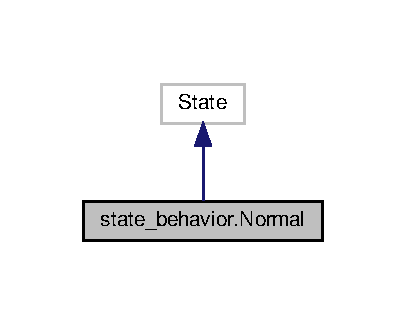
\includegraphics[width=195pt]{classstate__behavior_1_1Normal__inherit__graph}
\end{center}
\end{figure}


Collaboration diagram for state\+\_\+behavior.\+Normal\+:\nopagebreak
\begin{figure}[H]
\begin{center}
\leavevmode
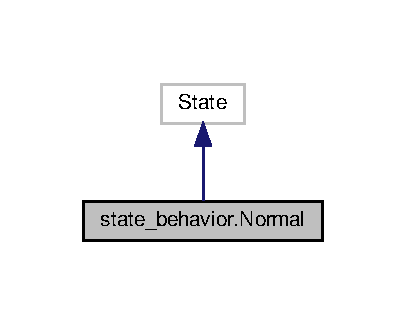
\includegraphics[width=195pt]{classstate__behavior_1_1Normal__coll__graph}
\end{center}
\end{figure}
\subsection*{Public Member Functions}
\begin{DoxyCompactItemize}
\item 
def \hyperlink{classstate__behavior_1_1Normal_a73b4aa2844d6c7f4b35bbb53cea791dd}{\+\_\+\+\_\+init\+\_\+\+\_\+} (self)
\begin{DoxyCompactList}\small\item\em {\bfseries init} initialises the \hyperlink{classstate__behavior_1_1Normal}{Normal} state in the smach\+\_\+state \end{DoxyCompactList}\item 
def \hyperlink{classstate__behavior_1_1Normal_ad34ac585f5ba450b5e2921bb69132f4d}{execute} (self, userdata)
\begin{DoxyCompactList}\small\item\em In this \hyperlink{classstate__behavior_1_1Normal_ad34ac585f5ba450b5e2921bb69132f4d}{execute()} function, the robot randomly walks in the environment until it reaches the tired\+\_\+level The logic used here is that if we receive a command play in the middle, it reaches the last coordinate and that is published in the rostopic /move\+To\+Pose and shifts to \hyperlink{classstate__behavior_1_1Play}{Play} state. \end{DoxyCompactList}\end{DoxyCompactItemize}
\subsection*{Public Attributes}
\begin{DoxyCompactItemize}
\item 
\mbox{\Hypertarget{classstate__behavior_1_1Normal_af8396ab1f88ae1ea117eab1702245e35}\label{classstate__behavior_1_1Normal_af8396ab1f88ae1ea117eab1702245e35}} 
{\bfseries pub}
\item 
\mbox{\Hypertarget{classstate__behavior_1_1Normal_af3a907e6ca2e16d50543abb06dc8e41c}\label{classstate__behavior_1_1Normal_af3a907e6ca2e16d50543abb06dc8e41c}} 
{\bfseries is\+Reached}
\item 
\mbox{\Hypertarget{classstate__behavior_1_1Normal_a9569665701706ec91ab67cb28f4ad231}\label{classstate__behavior_1_1Normal_a9569665701706ec91ab67cb28f4ad231}} 
{\bfseries command\+\_\+play}
\end{DoxyCompactItemize}


\subsection{Detailed Description}
This class defines the state of the state machine corresponding to the robot randomly moving in the 2D plane. 

It is a inheritance from smach and the state is added to the smach\+\_\+state. In this state the robot moves around randomly by subscribing to the rostopic /move\+To\+Pose. It has a function \hyperlink{classstate__behavior_1_1Normal_ad34ac585f5ba450b5e2921bb69132f4d}{execute()} providing the intended behavior. 

\subsection{Constructor \& Destructor Documentation}
\mbox{\Hypertarget{classstate__behavior_1_1Normal_a73b4aa2844d6c7f4b35bbb53cea791dd}\label{classstate__behavior_1_1Normal_a73b4aa2844d6c7f4b35bbb53cea791dd}} 
\index{state\+\_\+behavior\+::\+Normal@{state\+\_\+behavior\+::\+Normal}!\+\_\+\+\_\+init\+\_\+\+\_\+@{\+\_\+\+\_\+init\+\_\+\+\_\+}}
\index{\+\_\+\+\_\+init\+\_\+\+\_\+@{\+\_\+\+\_\+init\+\_\+\+\_\+}!state\+\_\+behavior\+::\+Normal@{state\+\_\+behavior\+::\+Normal}}
\subsubsection{\texorpdfstring{\+\_\+\+\_\+init\+\_\+\+\_\+()}{\_\_init\_\_()}}
{\footnotesize\ttfamily def state\+\_\+behavior.\+Normal.\+\_\+\+\_\+init\+\_\+\+\_\+ (\begin{DoxyParamCaption}\item[{}]{self }\end{DoxyParamCaption})}



{\bfseries init} initialises the \hyperlink{classstate__behavior_1_1Normal}{Normal} state in the smach\+\_\+state 


\begin{DoxyParams}{Parameters}
{\em outcomes} & are the possible transitions which are either it can go to normal ot play state \\
\hline
{\em input\+\_\+keys} & These are possible input of the state \\
\hline
{\em output\+\_\+keys} & These are possible outputs of the state. \\
\hline
\end{DoxyParams}


\subsection{Member Function Documentation}
\mbox{\Hypertarget{classstate__behavior_1_1Normal_ad34ac585f5ba450b5e2921bb69132f4d}\label{classstate__behavior_1_1Normal_ad34ac585f5ba450b5e2921bb69132f4d}} 
\index{state\+\_\+behavior\+::\+Normal@{state\+\_\+behavior\+::\+Normal}!execute@{execute}}
\index{execute@{execute}!state\+\_\+behavior\+::\+Normal@{state\+\_\+behavior\+::\+Normal}}
\subsubsection{\texorpdfstring{execute()}{execute()}}
{\footnotesize\ttfamily def state\+\_\+behavior.\+Normal.\+execute (\begin{DoxyParamCaption}\item[{}]{self,  }\item[{}]{userdata }\end{DoxyParamCaption})}



In this \hyperlink{classstate__behavior_1_1Normal_ad34ac585f5ba450b5e2921bb69132f4d}{execute()} function, the robot randomly walks in the environment until it reaches the tired\+\_\+level The logic used here is that if we receive a command play in the middle, it reaches the last coordinate and that is published in the rostopic /move\+To\+Pose and shifts to \hyperlink{classstate__behavior_1_1Play}{Play} state. 

Otherwise the robot goes to \char`\"{}\+Sleep\char`\"{} state after it gets tired 

The documentation for this class was generated from the following file\+:\begin{DoxyCompactItemize}
\item 
/home/rohit/\+Exp\+Robo\+Assignment/src/finite\+\_\+state\+\_\+machine/src/state\+\_\+behavior.\+py\end{DoxyCompactItemize}

\hypertarget{classstate__behavior_1_1Play}{}\section{state\+\_\+behavior.\+Play Class Reference}
\label{classstate__behavior_1_1Play}\index{state\+\_\+behavior.\+Play@{state\+\_\+behavior.\+Play}}


Inheritance diagram for state\+\_\+behavior.\+Play\+:\nopagebreak
\begin{figure}[H]
\begin{center}
\leavevmode
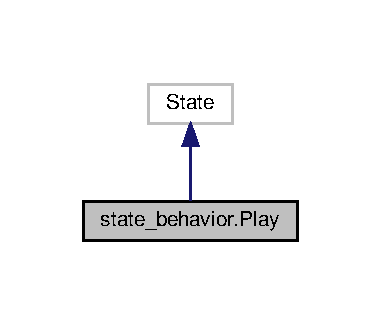
\includegraphics[width=183pt]{classstate__behavior_1_1Play__inherit__graph}
\end{center}
\end{figure}


Collaboration diagram for state\+\_\+behavior.\+Play\+:\nopagebreak
\begin{figure}[H]
\begin{center}
\leavevmode
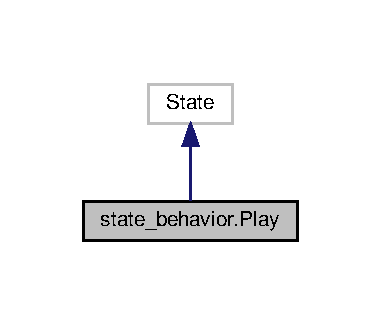
\includegraphics[width=183pt]{classstate__behavior_1_1Play__coll__graph}
\end{center}
\end{figure}
\subsection*{Public Member Functions}
\begin{DoxyCompactItemize}
\item 
def \hyperlink{classstate__behavior_1_1Play_af233d9d46accf0b314f2216d6add02ae}{\+\_\+\+\_\+init\+\_\+\+\_\+} (self)
\begin{DoxyCompactList}\small\item\em {\bfseries init} initializes the \hyperlink{classstate__behavior_1_1Play}{Play} state with the outcome go\+\_\+to\+\_\+normal. \end{DoxyCompactList}\item 
def \hyperlink{classstate__behavior_1_1Play_a0b3baf44027bc1d5ec262ea8b67063b9}{execute} (self, userdata)
\begin{DoxyCompactList}\small\item\em In this \hyperlink{classstate__behavior_1_1Play_a0b3baf44027bc1d5ec262ea8b67063b9}{execute()}, we implement play behavior. \end{DoxyCompactList}\end{DoxyCompactItemize}
\subsection*{Public Attributes}
\begin{DoxyCompactItemize}
\item 
\mbox{\Hypertarget{classstate__behavior_1_1Play_a0f0c471a70ad29733e9422a31adea20f}\label{classstate__behavior_1_1Play_a0f0c471a70ad29733e9422a31adea20f}} 
{\bfseries pub}
\end{DoxyCompactItemize}


\subsection{Constructor \& Destructor Documentation}
\mbox{\Hypertarget{classstate__behavior_1_1Play_af233d9d46accf0b314f2216d6add02ae}\label{classstate__behavior_1_1Play_af233d9d46accf0b314f2216d6add02ae}} 
\index{state\+\_\+behavior\+::\+Play@{state\+\_\+behavior\+::\+Play}!\+\_\+\+\_\+init\+\_\+\+\_\+@{\+\_\+\+\_\+init\+\_\+\+\_\+}}
\index{\+\_\+\+\_\+init\+\_\+\+\_\+@{\+\_\+\+\_\+init\+\_\+\+\_\+}!state\+\_\+behavior\+::\+Play@{state\+\_\+behavior\+::\+Play}}
\subsubsection{\texorpdfstring{\+\_\+\+\_\+init\+\_\+\+\_\+()}{\_\_init\_\_()}}
{\footnotesize\ttfamily def state\+\_\+behavior.\+Play.\+\_\+\+\_\+init\+\_\+\+\_\+ (\begin{DoxyParamCaption}\item[{}]{self }\end{DoxyParamCaption})}



{\bfseries init} initializes the \hyperlink{classstate__behavior_1_1Play}{Play} state with the outcome go\+\_\+to\+\_\+normal. 


\begin{DoxyParams}{Parameters}
{\em outcomes} & lists the possible transitions. From play we can go to normal state. \\
\hline
{\em input\+\_\+keys} & It is the possible input of the state  output keys It is the possible output of the state \\
\hline
\end{DoxyParams}


\subsection{Member Function Documentation}
\mbox{\Hypertarget{classstate__behavior_1_1Play_a0b3baf44027bc1d5ec262ea8b67063b9}\label{classstate__behavior_1_1Play_a0b3baf44027bc1d5ec262ea8b67063b9}} 
\index{state\+\_\+behavior\+::\+Play@{state\+\_\+behavior\+::\+Play}!execute@{execute}}
\index{execute@{execute}!state\+\_\+behavior\+::\+Play@{state\+\_\+behavior\+::\+Play}}
\subsubsection{\texorpdfstring{execute()}{execute()}}
{\footnotesize\ttfamily def state\+\_\+behavior.\+Play.\+execute (\begin{DoxyParamCaption}\item[{}]{self,  }\item[{}]{userdata }\end{DoxyParamCaption})}



In this \hyperlink{classstate__behavior_1_1Play_a0b3baf44027bc1d5ec262ea8b67063b9}{execute()}, we implement play behavior. 

A random position is generated for a person. The robot goes to the person, waits for the gesture and and goes to gesture position. the robot goes and comes back to the gesture position and waits for another gesture position until it gets tired. At last the robot goes to \hyperlink{classstate__behavior_1_1Normal}{Normal} position. 

The documentation for this class was generated from the following file\+:\begin{DoxyCompactItemize}
\item 
/home/rohit/\+Exp\+Robo\+Assignment/src/finite\+\_\+state\+\_\+machine/src/state\+\_\+behavior.\+py\end{DoxyCompactItemize}

\hypertarget{classstate__behavior_1_1Sleep}{}\section{state\+\_\+behavior.\+Sleep Class Reference}
\label{classstate__behavior_1_1Sleep}\index{state\+\_\+behavior.\+Sleep@{state\+\_\+behavior.\+Sleep}}


Inheritance diagram for state\+\_\+behavior.\+Sleep\+:\nopagebreak
\begin{figure}[H]
\begin{center}
\leavevmode
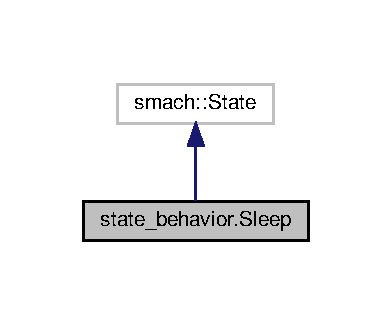
\includegraphics[width=188pt]{classstate__behavior_1_1Sleep__inherit__graph}
\end{center}
\end{figure}


Collaboration diagram for state\+\_\+behavior.\+Sleep\+:\nopagebreak
\begin{figure}[H]
\begin{center}
\leavevmode
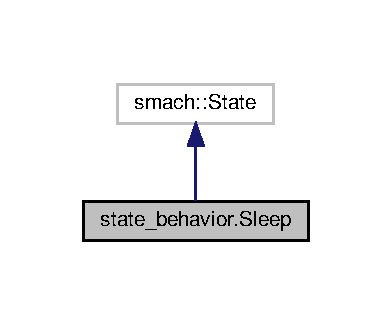
\includegraphics[width=188pt]{classstate__behavior_1_1Sleep__coll__graph}
\end{center}
\end{figure}
\subsection*{Public Member Functions}
\begin{DoxyCompactItemize}
\item 
def \hyperlink{classstate__behavior_1_1Sleep_a6550cf2697cc65d83162891ad194fe2d}{\+\_\+\+\_\+init\+\_\+\+\_\+} (self)
\begin{DoxyCompactList}\small\item\em {\bfseries init} initialises the \hyperlink{classstate__behavior_1_1Sleep}{Sleep} state in the smach\+\_\+state \end{DoxyCompactList}\item 
def \hyperlink{classstate__behavior_1_1Sleep_a79cf281b29f33265acc97354865a2f3c}{execute} (self, userdata)
\begin{DoxyCompactList}\small\item\em In this \hyperlink{classstate__behavior_1_1Sleep_a79cf281b29f33265acc97354865a2f3c}{execute()} function, the robot goes to predefined home\+\_\+fixed position The position is published in the topic /move\+To\+Pose The logic used here is that if we receive a command play in the middle, it reaches the last coordinate and that is published in the rostopic /move\+To\+Pose and shifts to \hyperlink{classstate__behavior_1_1Play}{Play} state. \end{DoxyCompactList}\end{DoxyCompactItemize}
\subsection*{Public Attributes}
\begin{DoxyCompactItemize}
\item 
\mbox{\Hypertarget{classstate__behavior_1_1Sleep_abd6af3621ac6fd6caab94e5ebd1d87ad}\label{classstate__behavior_1_1Sleep_abd6af3621ac6fd6caab94e5ebd1d87ad}} 
{\bfseries pub}
\item 
\mbox{\Hypertarget{classstate__behavior_1_1Sleep_a937ce4dfca4da54cb10ea6c00fa01bee}\label{classstate__behavior_1_1Sleep_a937ce4dfca4da54cb10ea6c00fa01bee}} 
{\bfseries is\+Reached}
\end{DoxyCompactItemize}


\subsection{Constructor \& Destructor Documentation}
\mbox{\Hypertarget{classstate__behavior_1_1Sleep_a6550cf2697cc65d83162891ad194fe2d}\label{classstate__behavior_1_1Sleep_a6550cf2697cc65d83162891ad194fe2d}} 
\index{state\+\_\+behavior\+::\+Sleep@{state\+\_\+behavior\+::\+Sleep}!\+\_\+\+\_\+init\+\_\+\+\_\+@{\+\_\+\+\_\+init\+\_\+\+\_\+}}
\index{\+\_\+\+\_\+init\+\_\+\+\_\+@{\+\_\+\+\_\+init\+\_\+\+\_\+}!state\+\_\+behavior\+::\+Sleep@{state\+\_\+behavior\+::\+Sleep}}
\subsubsection{\texorpdfstring{\+\_\+\+\_\+init\+\_\+\+\_\+()}{\_\_init\_\_()}}
{\footnotesize\ttfamily def state\+\_\+behavior.\+Sleep.\+\_\+\+\_\+init\+\_\+\+\_\+ (\begin{DoxyParamCaption}\item[{}]{self }\end{DoxyParamCaption})}



{\bfseries init} initialises the \hyperlink{classstate__behavior_1_1Sleep}{Sleep} state in the smach\+\_\+state 


\begin{DoxyParams}{Parameters}
{\em outcomes} & are the possible transition is it can to normal state by wake\+\_\+up transition \\
\hline
{\em input\+\_\+keys} & These are possible input of the state \\
\hline
{\em output\+\_\+keys} & These are possible outputs of the state. \\
\hline
\end{DoxyParams}


\subsection{Member Function Documentation}
\mbox{\Hypertarget{classstate__behavior_1_1Sleep_a79cf281b29f33265acc97354865a2f3c}\label{classstate__behavior_1_1Sleep_a79cf281b29f33265acc97354865a2f3c}} 
\index{state\+\_\+behavior\+::\+Sleep@{state\+\_\+behavior\+::\+Sleep}!execute@{execute}}
\index{execute@{execute}!state\+\_\+behavior\+::\+Sleep@{state\+\_\+behavior\+::\+Sleep}}
\subsubsection{\texorpdfstring{execute()}{execute()}}
{\footnotesize\ttfamily def state\+\_\+behavior.\+Sleep.\+execute (\begin{DoxyParamCaption}\item[{}]{self,  }\item[{}]{userdata }\end{DoxyParamCaption})}



In this \hyperlink{classstate__behavior_1_1Sleep_a79cf281b29f33265acc97354865a2f3c}{execute()} function, the robot goes to predefined home\+\_\+fixed position The position is published in the topic /move\+To\+Pose The logic used here is that if we receive a command play in the middle, it reaches the last coordinate and that is published in the rostopic /move\+To\+Pose and shifts to \hyperlink{classstate__behavior_1_1Play}{Play} state. 

Otherwise the robot goes to \char`\"{}\+Sleep\char`\"{} state after it gets tired 

The documentation for this class was generated from the following file\+:\begin{DoxyCompactItemize}
\item 
/home/rohit/\+Exp\+Robo\+Assignment/src/finite\+\_\+state\+\_\+machine/src/state\+\_\+behavior.\+py\end{DoxyCompactItemize}

\chapter{File Documentation}
\hypertarget{random__motion_8cpp}{}\section{/home/rohit/\+Exp\+Robo\+Assignment/src/robot\+\_\+motion/src/random\+\_\+motion.cpp File Reference}
\label{random__motion_8cpp}\index{/home/rohit/\+Exp\+Robo\+Assignment/src/robot\+\_\+motion/src/random\+\_\+motion.\+cpp@{/home/rohit/\+Exp\+Robo\+Assignment/src/robot\+\_\+motion/src/random\+\_\+motion.\+cpp}}
{\ttfamily \#include $<$sstream$>$}\newline
{\ttfamily \#include $<$stdio.\+h$>$}\newline
{\ttfamily \#include $<$iostream$>$}\newline
{\ttfamily \#include $<$stdlib.\+h$>$}\newline
{\ttfamily \#include \char`\"{}ros/ros.\+h\char`\"{}}\newline
{\ttfamily \#include $<$std\+\_\+msgs/\+Int16.\+h$>$}\newline
{\ttfamily \#include $<$geometry\+\_\+msgs/\+Point.\+h$>$}\newline
{\ttfamily \#include $<$std\+\_\+msgs/\+Bool.\+h$>$}\newline
Include dependency graph for random\+\_\+motion.\+cpp\+:\nopagebreak
\begin{figure}[H]
\begin{center}
\leavevmode
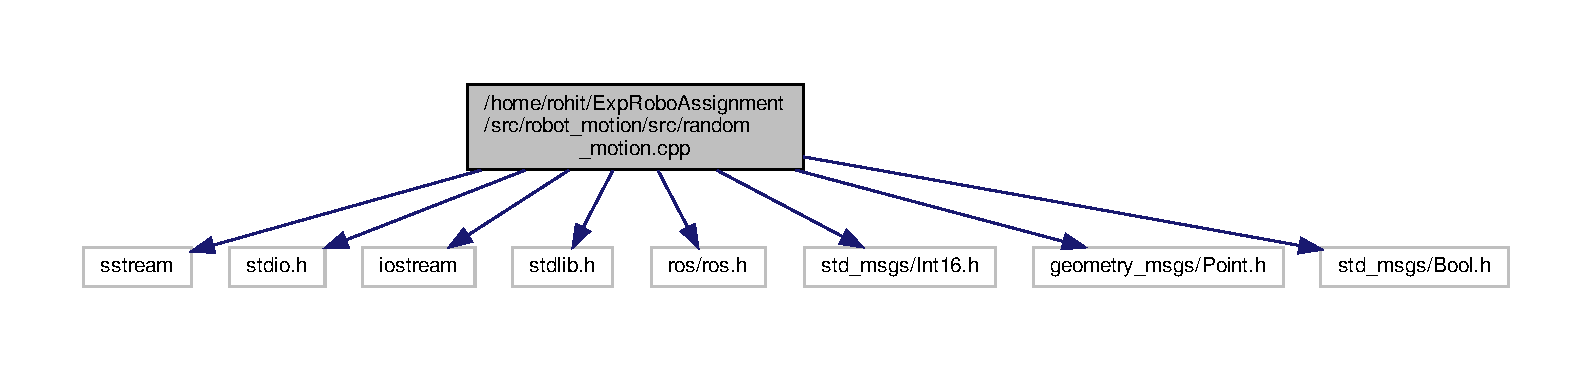
\includegraphics[width=350pt]{random__motion_8cpp__incl}
\end{center}
\end{figure}
\subsection*{Functions}
\begin{DoxyCompactItemize}
\item 
void \hyperlink{random__motion_8cpp_aad593c86a4f2bd1ff9f0fc321583c0d5}{pos\+Callback} (geometry\+\_\+msgs\+::\+Point \+\_\+point)
\begin{DoxyCompactList}\small\item\em pos\+Callback function listens to the topic /move\+To\+Pos. It records the postions to be reached. The fucntion then declares that the positon is reached to be published on the topic /\+Rested \end{DoxyCompactList}\item 
int \hyperlink{random__motion_8cpp_a3c04138a5bfe5d72780bb7e82a18e627}{main} (int argc, char $\ast$$\ast$argv)
\begin{DoxyCompactList}\small\item\em In this funciton we listen subscribe to rostopic /move\+To\+Pose and publishes to rostopic /\+Reached. The idea here is that we say the robot has reached the position only after the robot has reahced the target. \end{DoxyCompactList}\end{DoxyCompactItemize}
\subsection*{Variables}
\begin{DoxyCompactItemize}
\item 
geometry\+\_\+msgs\+::\+Point \hyperlink{random__motion_8cpp_a481fb0076093985fd795ac2a67b47468}{move\+\_\+coord}
\item 
\mbox{\Hypertarget{random__motion_8cpp_a46260f4238c3b1e06271009e83cf6c96}\label{random__motion_8cpp_a46260f4238c3b1e06271009e83cf6c96}} 
std\+\_\+msgs\+::\+Bool {\bfseries position\+\_\+reached}
\item 
\mbox{\Hypertarget{random__motion_8cpp_abdd9b1bae9f506cf5a415e5af7d17493}\label{random__motion_8cpp_abdd9b1bae9f506cf5a415e5af7d17493}} 
bool {\bfseries reached\+\_\+} = false
\end{DoxyCompactItemize}


\subsection{Detailed Description}
\begin{DoxyAuthor}{Author}
Rohit Kumar (\href{mailto:rohitkb114@gmail.com}{\tt rohitkb114@gmail.\+com}) 
\end{DoxyAuthor}
\begin{DoxyVersion}{Version}
0.\+1 
\end{DoxyVersion}
\begin{DoxyDate}{Date}
2020-\/11-\/13
\end{DoxyDate}
\begin{DoxyCopyright}{Copyright}
Copyright (c) 2020 
\end{DoxyCopyright}


\subsection{Function Documentation}
\mbox{\Hypertarget{random__motion_8cpp_a3c04138a5bfe5d72780bb7e82a18e627}\label{random__motion_8cpp_a3c04138a5bfe5d72780bb7e82a18e627}} 
\index{random\+\_\+motion.\+cpp@{random\+\_\+motion.\+cpp}!main@{main}}
\index{main@{main}!random\+\_\+motion.\+cpp@{random\+\_\+motion.\+cpp}}
\subsubsection{\texorpdfstring{main()}{main()}}
{\footnotesize\ttfamily int main (\begin{DoxyParamCaption}\item[{int}]{argc,  }\item[{char $\ast$$\ast$}]{argv }\end{DoxyParamCaption})}



In this funciton we listen subscribe to rostopic /move\+To\+Pose and publishes to rostopic /\+Reached. The idea here is that we say the robot has reached the position only after the robot has reahced the target. 


\begin{DoxyParams}{Parameters}
{\em argc} & \\
\hline
{\em argv} & \\
\hline
\end{DoxyParams}
\begin{DoxyReturn}{Returns}
int 
\end{DoxyReturn}
\mbox{\Hypertarget{random__motion_8cpp_aad593c86a4f2bd1ff9f0fc321583c0d5}\label{random__motion_8cpp_aad593c86a4f2bd1ff9f0fc321583c0d5}} 
\index{random\+\_\+motion.\+cpp@{random\+\_\+motion.\+cpp}!pos\+Callback@{pos\+Callback}}
\index{pos\+Callback@{pos\+Callback}!random\+\_\+motion.\+cpp@{random\+\_\+motion.\+cpp}}
\subsubsection{\texorpdfstring{pos\+Callback()}{posCallback()}}
{\footnotesize\ttfamily void pos\+Callback (\begin{DoxyParamCaption}\item[{geometry\+\_\+msgs\+::\+Point}]{\+\_\+point }\end{DoxyParamCaption})}



pos\+Callback function listens to the topic /move\+To\+Pos. It records the postions to be reached. The fucntion then declares that the positon is reached to be published on the topic /\+Rested 


\begin{DoxyParams}{Parameters}
{\em \+\_\+point} & It takes the argument as point after subscribing to the topic /move\+To\+Pose \\
\hline
\end{DoxyParams}


\subsection{Variable Documentation}
\mbox{\Hypertarget{random__motion_8cpp_a481fb0076093985fd795ac2a67b47468}\label{random__motion_8cpp_a481fb0076093985fd795ac2a67b47468}} 
\index{random\+\_\+motion.\+cpp@{random\+\_\+motion.\+cpp}!move\+\_\+coord@{move\+\_\+coord}}
\index{move\+\_\+coord@{move\+\_\+coord}!random\+\_\+motion.\+cpp@{random\+\_\+motion.\+cpp}}
\subsubsection{\texorpdfstring{move\+\_\+coord}{move\_coord}}
{\footnotesize\ttfamily geometry\+\_\+msgs\+::\+Point move\+\_\+coord}

These are R\+OS specific headers $<$ Integer related headers Header required for geometry\+\_\+messages 
%--- End generated contents ---

% Index
\backmatter
\newpage
\phantomsection
\clearemptydoublepage
\addcontentsline{toc}{chapter}{Index}
\printindex

\end{document}
